% 双摆和三摆
% 拉格朗日方程|混沌|三摆

\pentry{拉格朗日方程\upref{Lagrng}}

\subsection{双摆}
 (未完成)

\subsection{三摆}
\begin{figure}[ht]
\centering
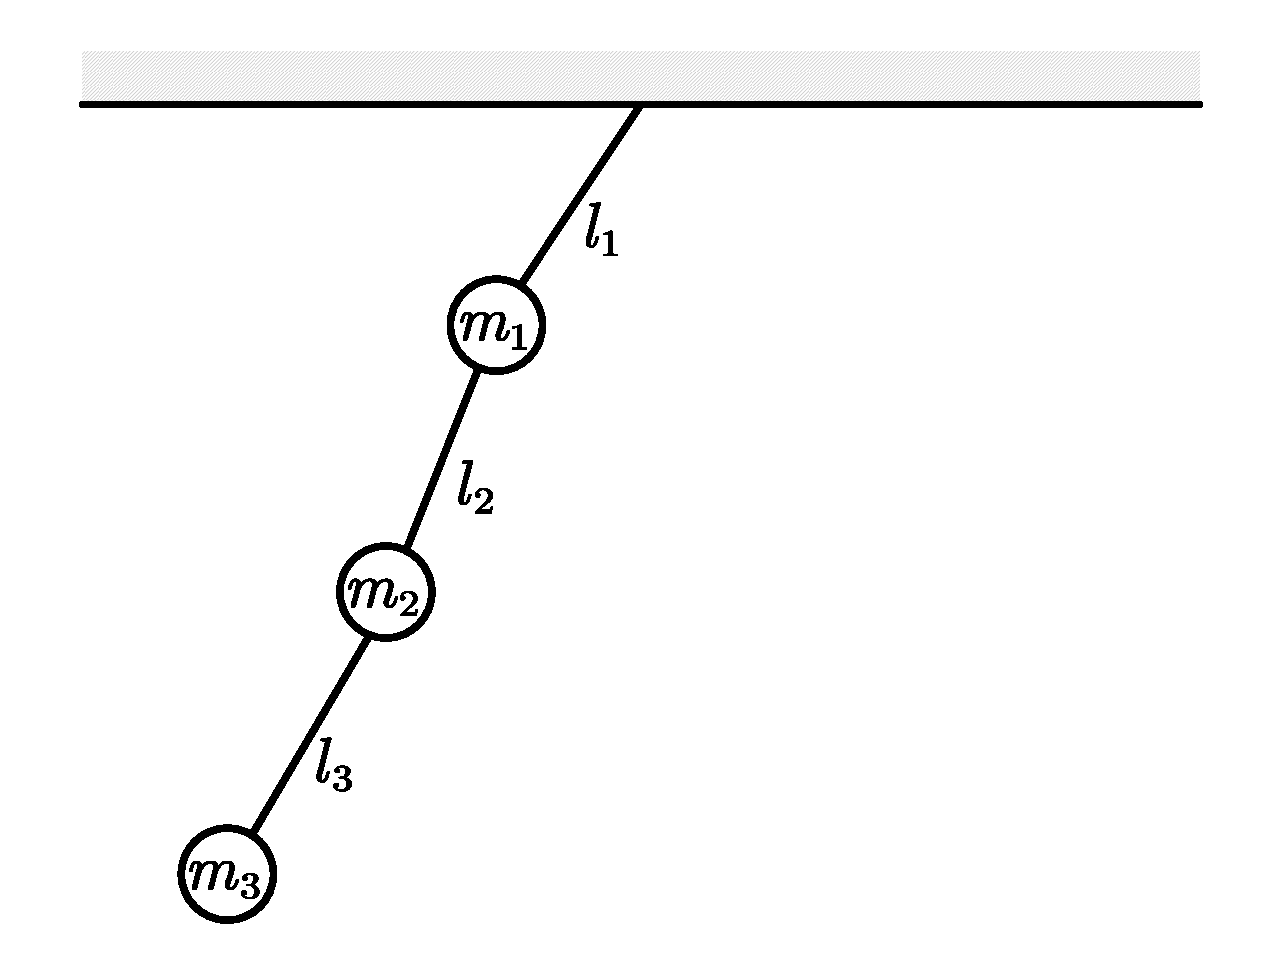
\includegraphics[width=8cm]{./figures/Pendu3_1.pdf}
\caption{三摆} \label{Pendu3_fig1}
\end{figure}
如\autoref{Pendu3_fig1} 所示,三根质量不计的杆长度分别为 $l_1, l_2, l_3$, 三个质点的质量分别为 $m_1, m_2, m_3$. 我们把这个模型叫做\textbf{三摆}. 三摆常用于演示物理学中的混沌现象.
\subsubsection{运动方程}
 
\begin{equation}
\begin{aligned}
T &= \frac{1}{2} m_1 (l_1 \omega_1)^2 + \frac{1}{2} m_2 [(l_1 \omega_1 \cos\theta_1 + l_2 \omega_2 \cos\theta_2)^2 +\\
&\qquad \qquad\qquad\qquad\qquad\qquad (l_1 \omega_1 \sin\theta_1 + l_2 \omega_2 \sin\theta_2)^2]\\
& + \frac{1}{2} m_3 [(l_1 \omega_1 \cos\theta_1 + l_2 \omega_2 \cos\theta_2 + l_3 \omega_3 \cos \theta_3)^2 +\\
&\qquad\qquad\qquad (l_1 \omega_1 \sin\theta_1 + l_2 \omega_2 \sin\theta_2 + l_3 \omega_3 \sin\theta_3)^2]
\end{aligned}
\end{equation}

\begin{equation} 
\begin{aligned} 
V &= -m_1 g l_1 \cos \theta_1 - m_2 g (l_1\cos \theta_1 + l_2 \cos \theta_2)\\
&\qquad - m_3 g (l_1 \cos\theta_1 + l_2 \cos \theta_2 + l_3 \cos \theta_3)
\end{aligned}
\end{equation}

\begin{equation}
L(\theta_1, \theta_2, \theta_3, \omega_1, \omega_2, \omega_3) = T(\omega_1, \omega_2, \omega_3) - V(\theta_1, \theta_2, \theta_3)
\end{equation}

\begin{equation}
\dv{t} \pdv{L}{\omega_i} = \pdv{L}{\theta_i} \quad (i=1,2,3)
\end{equation}

这是一个二阶微分方程组.

% 未完成: 数值解, 程序, 动画

